% CVPR 2025 Paper Template; see https://github.com/cvpr-org/author-kit

\documentclass[10pt,twocolumn,letterpaper]{article}

%%%%%%%%% PAPER TYPE  - PLEASE UPDATE FOR FINAL VERSION
\usepackage{cvpr}              % To produce the CAMERA-READY version
% \usepackage[review]{cvpr}      % To produce the REVIEW version
% \usepackage[pagenumbers]{cvpr} % To force page numbers, e.g. for an arXiv version

% Import additional packages in the preamble file, before hyperref
%
% --- inline annotations
%
\newcommand{\red}[1]{{\color{red}#1}}
\newcommand{\todo}[1]{{\color{red}#1}}
\newcommand{\TODO}[1]{\textbf{\color{red}[TODO: #1]}}
% --- disable by uncommenting  
% \renewcommand{\TODO}[1]{}
% \renewcommand{\todo}[1]{#1}



% It is strongly recommended to use hyperref, especially for the review version.
% hyperref with option pagebackref eases the reviewers' job.
% Please disable hyperref *only* if you encounter grave issues, 
% e.g. with the file validation for the camera-ready version.
%
% If you comment hyperref and then uncomment it, you should delete *.aux before re-running LaTeX.
% (Or just hit 'q' on the first LaTeX run, let it finish, and you should be clear).
\definecolor{cvprblue}{rgb}{0.21,0.49,0.74}
\usepackage[pagebackref,breaklinks,colorlinks,allcolors=cvprblue]{hyperref}

\usepackage{algorithm}
\usepackage{algpseudocode}
\usepackage{tabularx}
\usepackage{adjustbox}
\usepackage{amsmath}
\usepackage{multirow} 
\usepackage{graphicx}
\usepackage{caption}

%%%%%%%%% PAPER ID  - PLEASE UPDATE
\def\paperID{*****} % *** Enter the Paper ID here
\def\confName{CVPR}
\def\confYear{2025}

%%%%%%%%% TITLE
\title{Assignment 3: RNN Stock Price Prediction}

%%%%%%%%% AUTHORS
\author{Caleb Rust\\
The University of Adelaide\\
{\tt\small a1782615@adelaide.edu.au}
}

\begin{document}
\maketitle
\begin{abstract}
This assignment explores the application of LSTM-based recurrent neural networks for stock price prediction, focusing on Google's stock due to its high trading volume and extensive data availability. The model leverages a rolling window approach with z-score standardization for input preprocessing and employs a naive trading strategy to evaluate prediction performance. Experiments were conducted to assess the impact of architectural variations, hyperparameters, and loss functions on prediction accuracy. While the LSTM demonstrated potential, significant overfitting to the training data and an inability to generalize to test data with higher price ranges highlighted key limitations. Suggestions for future improvements include enhanced preprocessing techniques, data augmentation, and more sophisticated trading strategies.
\end{abstract}
    
\section{Introduction}
\label{sec:intro}

The goal of this assigment is to use RNNs to predict stock prices and implement a simple trading strategy based on these predictions. 

Google's stock \cite{goog} was chosen as the target stock due to its high trading volume and the availability of data. 

The LSTM model architecture was chosen due to its ability to capture long-term dependencies in sequential data and it's handling of vanishing gradients. LSTM models have been shown to be effective in time series forecasting tasks\cite{lstm}.

Accompanying notebook is available at \url{https://github.com/redrusty2/<bla>}.

\section{Method} \label{sec:method}

\subsection{Dataset}

The dataset consists of daily Google stock data sourced from \textit{Yahoo Finance}\cite{goog} with the \textit{yfinance} Python package\cite{yfinance}, spanning from 2004 to 2019. The features include the closing, high, low, and opening prices, as well as trading volume and the date. The dataset was divided into training and testing subsets, with the training portion further split into separate training and validation sets. All features were standardised using the z-score method, with the mean and standard deviation estimated from the training set and subsequently applied to the test set. Z-score was used to make sure the model can generalise to values outside the range of the training set.

2019 was chosen as the endpoint since the COVID-19 pandemic caused significant market fluctuations, which could potentially skew the model’s performance. 

The test set was chosen to be the last 15\% of the data, the validation set was chosen to be the last 15\% of the training set, and the training set was the remaining 72.25\% of the data.

\subsection{Strategy}

The trading strategy involves examining the predicted price three days into the future on each day. If the model forecasts a higher price compared to the current one, a fixed quantity of the stock is purchased and held until the third day, at which point it is sold. If the prediction indicates a lower price, no action is taken. The total return percentage is calculated by summing the return percentage from each trade.

For example if 3 trades are made with returns of 10\%, 5\%, and 2\%, the total return would be 17\%.

This is a very naive strategy and does not take into account transaction costs, slippage, or other factors that would be present in a real-world scenario but gives a good starting point.

\subsection{Model}

The model\cite{rnn_pytorch} is based on an LSTM architecture followed by a fully connected (FC) layer. The LSTM receives the feature set and produces representations that the FC layer uses to output the future close, open, high, low, and volume predictions. Multiple configurations of the LSTM were explored, including varying the number of layers, hidden layer sizes, and the choice of which outputs (entire sequence, final time step) were fed into the FC layer.

All models were implemented with 5 input features and 5 output features per day.  

2 versions of the model were tested. One where the entire LSTM output sequence was fed into the FC layer and one where only the final hidden state was fed into the FC layer.

Multiple layers were also tested. This is where the output of the LSTM is fed into another LSTM layer. This was tested with 1 and 2 layers. Dropout was added to the final LSTM layer when using multiple layers to prevent overfitting.

\subsubsection{Training}

A rolling window of 30 days was employed to predict the stock price three days ahead. Each window’s prediction was generated using overlapping windows shifted by one day. For each prediction, the model outputs the close, open, high, low, and volume values three days in the future. 

Windows are shuffled and batched

In order to get the model to output 3 future values and auto-regressive approach was used. 
For each window, the model is first given the 30 day window as input and predicts a single day. The predicted day is then appended to the 30 day input and the these 31 days are used as input. This is repeated until 3 days are predicted. 

\subsubsection{Loss}

Various loss functions were tested to improve training stability and accuracy, including Mean Squared Error (MSE), Mean Absolute Error (MAE, L1Loss), and the Huber loss(SmoothL1Loss).

MSE is sensitive to outliers while MAE is not. Huber loss is the combination of both\cite{loss_functions}. 

\subsubsection{Optimiser}

The Adam optimiser was used to train the model. A weight decay of $1 \times 10^{-5}$ was applied to the optimiser to prevent overfitting for all experiments.

\subsubsection{Early Stopping}

The model was trained for up to 2000 epochs, though this upper limit was never reached due to early stopping criteria. After each epoch, the validation loss was evaluated. Whenever the validation loss improved, the model parameters were saved as a checkpoint. If the validation loss did not improve for 50 consecutive epochs, the training process was halted, and the best checkpoint was restored for subsequent evaluation and inference on the test set.


\section{Experiments}

Initial experiments involved using the entire LSTM output sequence as input to the FC layer. This approach resulted in unusable predictions, with the model often producing unrealistic price jumps between consecutive predictions. Adjusting the loss function, model size, and other hyperparameters did not resolve this issue. Switching from using the entire LSTM output to the last single LSTM output led to more stable predictions. 

\begin{figure}[h]
    \centering
    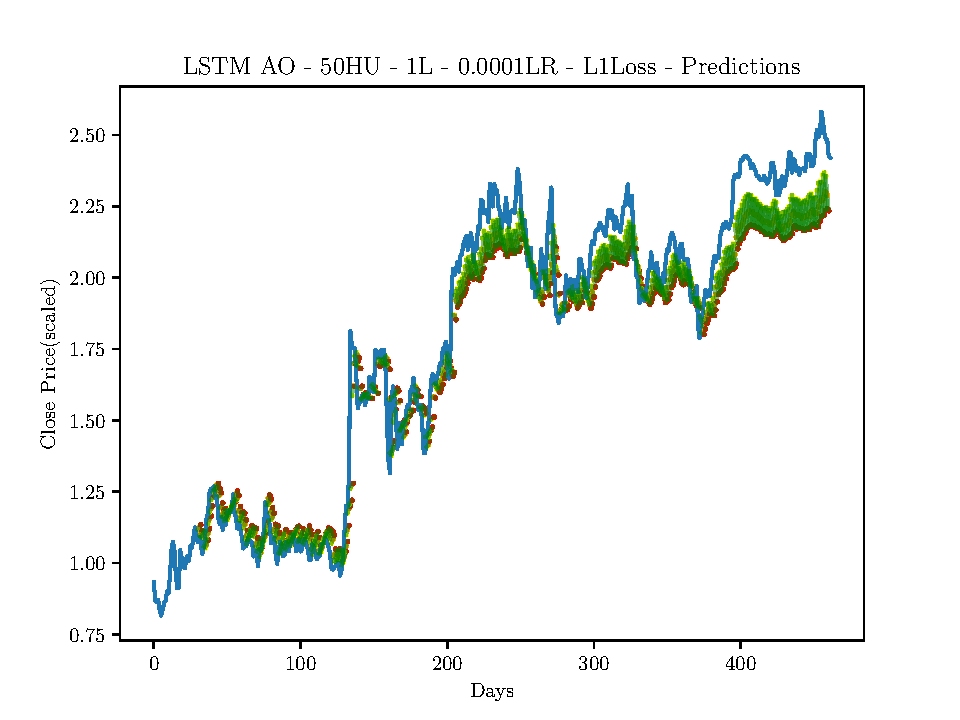
\includegraphics[width=0.5\textwidth, trim=20 0 20 10, clip]{plots/LSTM AO - 50HU - 1L - 0.0001LR - L1Loss-predictions.pdf}
    \caption{Predictions of the model with 50 hidden units and 1 layer. Green lines represent the predictions, red markers indicate the 3 predicted day.}
    \label{fig:ao_50HU_1L}
\end{figure}

\begin{figure}[h]
    \centering
    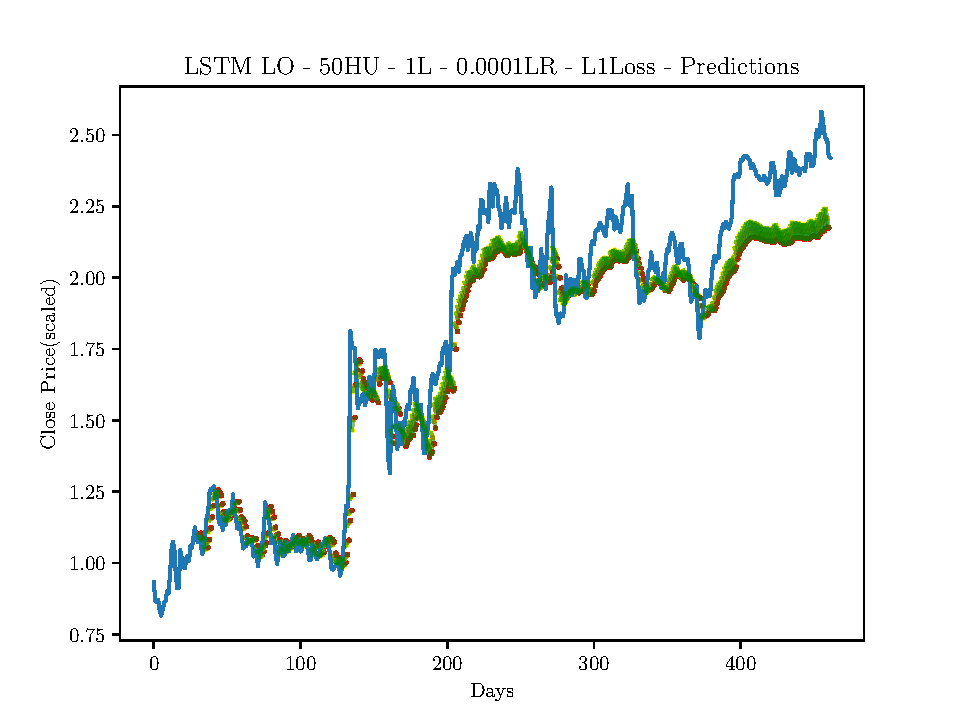
\includegraphics[width=0.5\textwidth, trim=20 0 20 10, clip]{plots/LSTM LO - 50HU - 1L - 0.0001LR - L1Loss-predictions.pdf}
    \caption{Predictions of the model with 50 hidden units and 1 layer. Green lines represent the predictions, red markers indicate the 3 predicted day.}
    \label{fig:lo_50HU_1L}
\end{figure}


The experiments started with the following hyperparameters: 5 input features, 5 output features, 50 hidden units, 1 layer, L1 loss, 0.0001 learning rate(LR), 1e-5 weight decay. Both model varients for 50 hidden units can be viewed in Figure \ref{fig:ao_50HU_1L} and Figure \ref{fig:lo_50HU_1L}.

\begin{figure}[h]
    \centering
    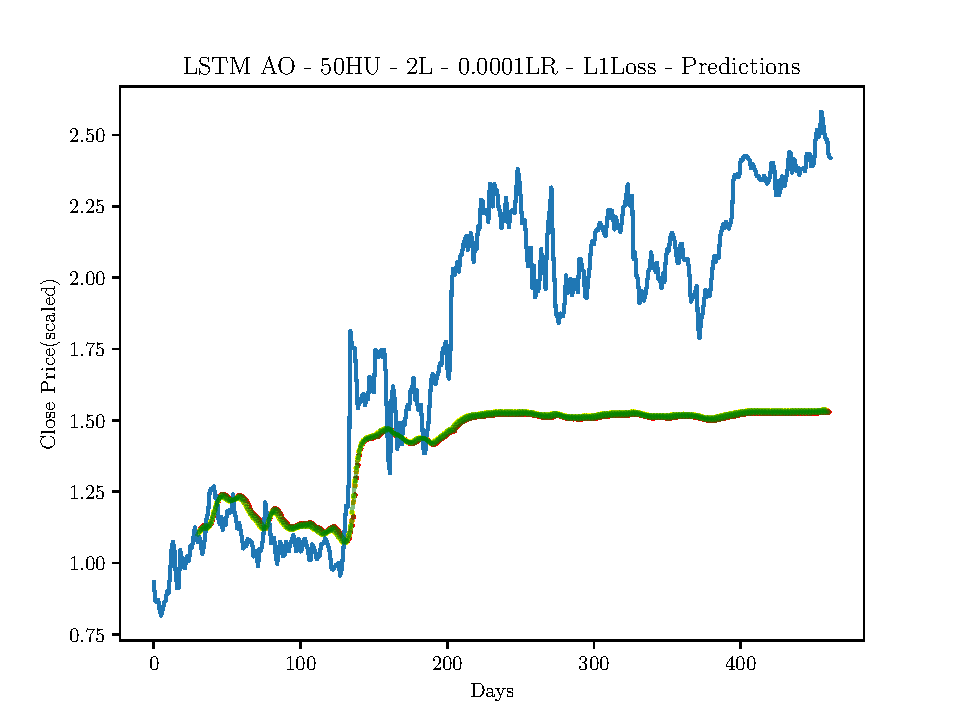
\includegraphics[width=0.5\textwidth, trim=20 0 20 10, clip]{plots/LSTM AO - 50HU - 2L - 0.0001LR - L1Loss-predictions.pdf}
    \caption{Predictions of the model with 50 hidden units and 2 layers. Green lines represent the predictions, red markers indicate the 3 predicted day. The predictions are smoothed out too much and resemble a moving average.}
    \label{fig:smoothed_out}
\end{figure}

Using 2 or more layers resulted in the predictions being smoothed out too much, see Figure \ref{fig:smoothed_out}, and resembles a moving average. This also caused no buys to be made with the strategy as time progressed since the Google stock price increases over time. The quality of the predictions do not look good as once the price gets high, the model always predicts the price to decrease.

As can be seen in Table \ref{tab:results}, 20 hidden units has a higher loss but performs well with the strategy. 50 and 100 hidden units have a lower loss but perform worse with the strategy. This is likely due to the model overfitting to the training data.

L1Loss seems to be important for the model to perform well. In Table \ref{tab:results}, L1Loss performed the best for the LSTM using the last output, while SmoothL1Loss(which is L1Loss \& MSELoss) performed the best for the LSTM using the entire output. MSELoss performed the worst in all cases. Note we can not compare the loss values directly between the different loss functions as they are calculated differently.

All the model variations converged well during training with a smooth loss curve, see Figure \ref{fig:loss_curve}. But it can also be seen that the model is heavily overfitting to the training data. Weight decay alone was not enough to prevent this.

\begin{figure}[h]
    \centering
    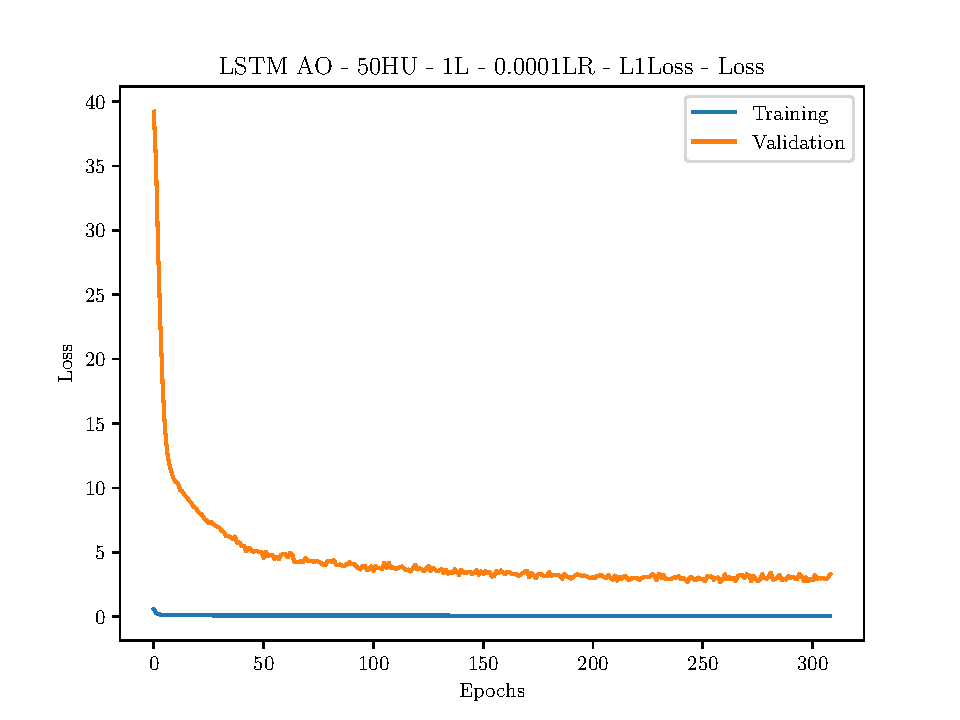
\includegraphics[width=0.5\textwidth, trim=20 0 20 10, clip]{plots/LSTM AO - 50HU - 1L - 0.0001LR - L1Loss-loss.pdf}
    \caption{Loss curve of the model with 50 hidden units and 1 layer.}
    \label{fig:loss_curve}
\end{figure}

\begin{table}[h]
    \centering
    \begin{tabular}{lcc}
        \hline
        \textbf{Model} & \textbf{Val. Loss} & \textbf{Return(\%)} \\ \hline
        w/all 100HU & 2.71 & 57 \\ 
        w/all 50HU & 2.66 & 71 \\ 
        w/all 20HU & 3.63 & 89 \\
        \hline
        w/last 100HU & 2.38 & 75 \\
        w/last 50HU & 2.84 & 53 \\
        w/last 20HU & 3.92 & 82 \\
        \hline
        w/all 50HU 1L & 2.66 & 71 \\ 
        w/all 50HU 2L & 8.99 & 71 \\ 
        \hline
        w/last 50HU 1L & 2.84 & 53 \\
        w/last 50HU 2L & 9.22 & 48 \\ 
        \hline
        w/all 100HU L1Loss & 2.71 & 57 \\ 
        w/all 100HU MSELoss & 1.04 & 41 \\ 
        w/all 100HU SmoothL1Loss & 0.42 & 77 \\ 
        \hline
        w/last 100HU L1Loss & 2.38 & 75 \\ 
        w/last 100HU MSELoss & 1.41 & 58 \\ 
        w/last 100HU SmoothL1Loss & 0.41 & 64 \\ 
    \end{tabular}
    \caption{Results of hyperparameter tuning. HU = Hidden Units, L = Layers, w/all = entire LSTM output, w/last = final hidden state. If not stated, assume 1L and L1Loss}
    \label{tab:results}
\end{table}

\begin{figure}[h]
    \centering
    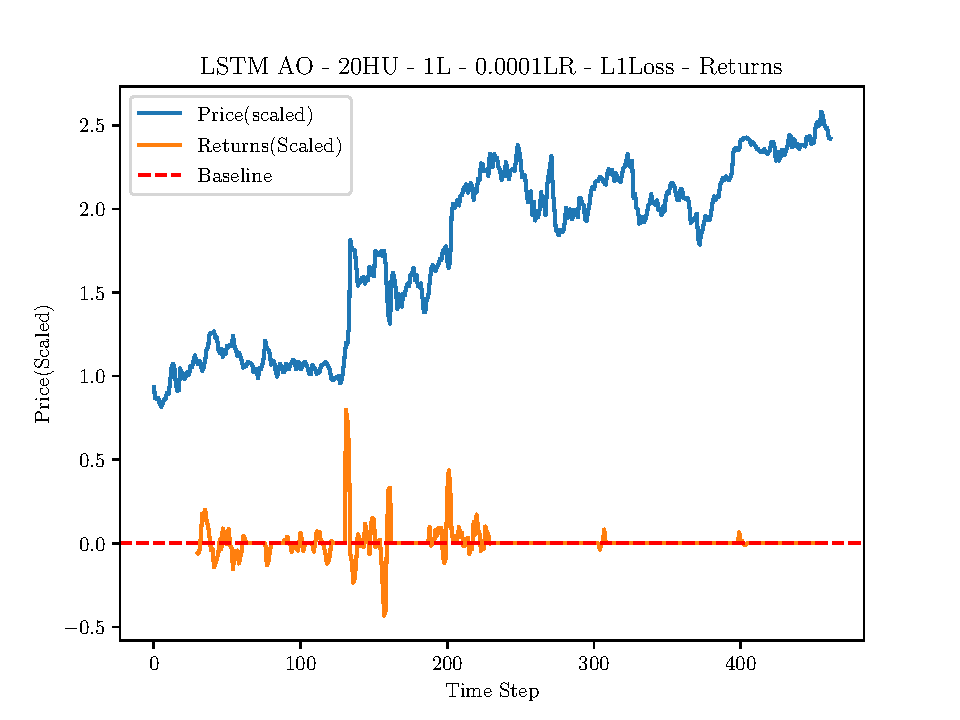
\includegraphics[width=0.5\textwidth, trim=20 0 20 10, clip]{plots/LSTM AO - 20HU - 1L - 0.0001LR - L1Loss-returns.pdf}
    \caption{Returns of the model with 20 hidden units and 1 layer. Although the model has the highest return, it does not handle stock prices that are much higher than the training data.}
    \label{fig:20HU_1L_returns}
\end{figure}

\begin{figure}[h]
    \centering
    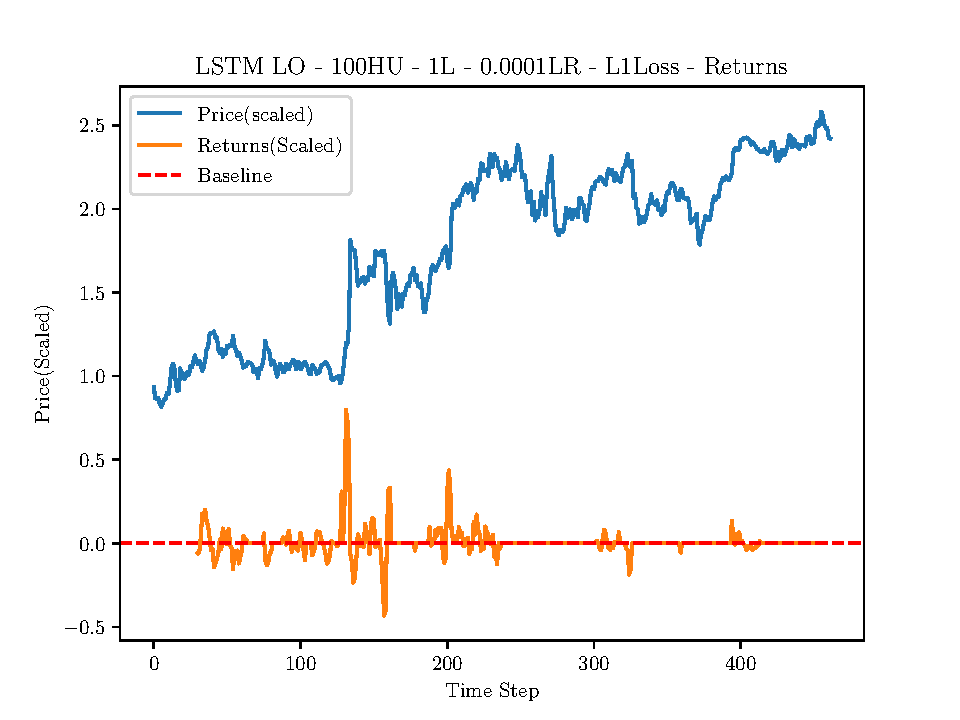
\includegraphics[width=0.5\textwidth, trim=20 0 20 10, clip]{plots/LSTM LO - 100HU - 1L - 0.0001LR - L1Loss-returns.pdf}
    \caption{Returns of the model with 20 hidden units and 1 layer. Does not perform as well as the 20 hidden unit model but does manage to make some successful trades at higher prices.}
    \label{fig:100HU_1L_returns}
\end{figure}

While the 20 hidden unit model did perform the best with the strategy, the loss was higher and upon inspection of the returns plot(Figure \ref{fig:20HU_1L_returns}), it can be seen that this model does not handle stock prices that are much higher than the training data. The 100 hidden unit models(Figure \ref{fig:100HU_1L_returns}) perform worse but do manage to make some successful trades at these higher prices. For this reason I am choosing the w/last 100HU 1L L1Loss model as the model to test on the test set.

\subsection{Final Test}

\begin{figure}[h]
    \centering
    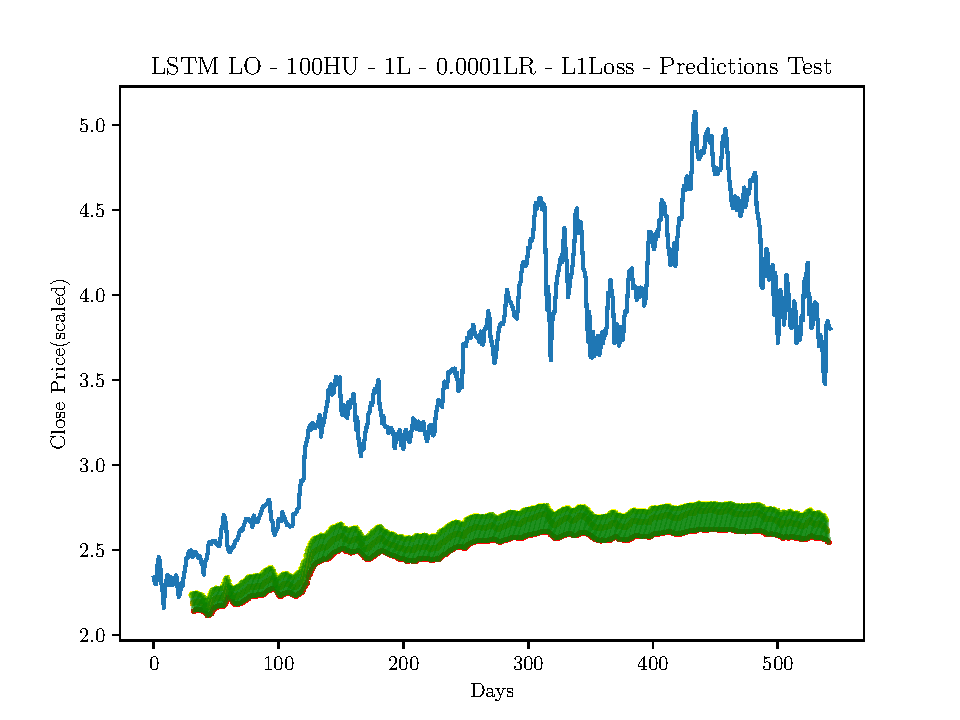
\includegraphics[width=0.5\textwidth, trim=20 0 20 10, clip]{plots/LSTM LO - 100HU - 1L - 0.0001LR - L1Loss-predictions-test.pdf}
    \caption{Predictions of the w/last 100HU 1L L1Loss model on the test set. Standardised prices in the test set are still too high relative to the training set for the model to be useful.}
    \label{fig:test_predtictions}
\end{figure}

The final test was conducted on the test set using the w/last 100HU 1L L1Loss model. Unfortunately, the model was a complete failure since the prices in the test set were much higher than the training set(Figure \ref{fig:test_predtictions}). Even though the dataset was standardised, the prices were so much higher(values of 4 - 5 after standardisation) that the model always predicted the price to decrease. After getting this result, I attempted to run the other models on the test set to see if any of them would work. Unfortunately, none of the models worked on the test set.


\section{Conclusion}

This assignment aimed to predict stock prices using an LSTM model to facilitate a simple but successful trading strategy. Unfortunately, the final model architecture, data preprocessing, and hyperparameters did not produce a model that could predict stock prices effectively. The model was heavily overfitting to the training data and could not generalise to the test set. The model was unable to handle stock prices that were much higher than the training data.

I think the main problem comes from the data preprocessing. The dataset was standardised using the z-score method, with the mean and standard deviation estimated from the training set and subsequently applied to the test set. Although this method is useful when inference inputs could be outside the range of the training set, it still does not handle the case where the values are much higher than the training set. I think a better strategy might be to use a smaller training set or normalise the data using a different method. 

Overfitting was another issue. Data augmentation could help here, either by adding noise to the data or by creating some synthetic data.

The strategy used was also very naive and did not take into account transaction costs, slippage, or other factors that would be present in a real-world scenario. A more sophisticated strategy could be used to improve the model's performance.





\section{Conclusion}

Data augmentation



{
    \small
    \bibliographystyle{ieeenat_fullname}
    \bibliography{main}
}

% WARNING: do not forget to delete the supplementary pages from your submission 
% \input{sec/X_suppl}

\end{document}

\input
